\documentclass[12pt,a4paper]{ctexart}

% 页面设置
\usepackage{geometry}
\geometry{left=2.5cm,right=2.5cm,top=2.5cm,bottom=2.5cm}

% 字体与行距
\setCJKmainfont{Noto Serif CJK SC}
\setmainfont{Times New Roman} % 英文正文 Times New Roman
\linespread{1.5}
\setlength{\parindent}{2em}
\setlength{\parskip}{0pt}

% 列表格式
\usepackage{enumitem}
\setlist[itemize]{noitemsep, topsep=2pt}
\setlist[enumerate]{noitemsep, topsep=2pt}

% 图形
\usepackage{graphicx}
\usepackage{float}
\usepackage{tikz}
\usetikzlibrary{arrows.meta, positioning, shapes.geometric}

% 超链接
\usepackage{hyperref}
\hypersetup{colorlinks=true, linkcolor=black, urlcolor=blue}

% 章节标题格式
\ctexset{
  section={format=\zihao{3}\heiti\bfseries\centering, beforeskip=0.5\baselineskip, afterskip=0.5\baselineskip},
  subsection={format=\zihao{4}\heiti\bfseries, beforeskip=0.5\baselineskip, afterskip=0.5\baselineskip},
  subsubsection={format=\zihao{-4}\heiti\bfseries, beforeskip=0.5\baselineskip, afterskip=0.5\baselineskip}
}

% 自定义命令
\newcommand{\todo}[1]{\textcolor{red}{\textbf{【待补充：#1】}}}
\newcommand{\code}[1]{\texttt{#1}}





\title{RISC-V CPU 上板验证报告}
\author{姓名：李建昊\\院校：上海科技大学\\专业：电子信息工程}
\date{2026年5月7日}

\begin{document}

% \maketitle
% \newpage
\tableofcontents
\newpage

\section{验证平台说明}
\subsection{FPGA平台型号}
本次上板验证使用竞业达 JYD FPGA 数字孪生平台。Vivado 工程目标器件为 Xilinx Kintex-7 系列，具体器件型号为 \code{xc7k325tffg900-2}。自研 CPU 顶层模块接入企业模板中的 \code{Core\_cpu} 位置，通过独立 IROM 接口完成取指，并通过统一的 \code{perip} 接口访问 DRAM、LED、七段数码管和计数器等外设。

本设计实现的是基于 RV32I 基本整数指令集的 32 位五级流水线 CPU。流水线划分为 IF、ID、EX、MEM、WB 五级，包含 PC/NPC、控制器、立即数生成、寄存器堆、ALU、访存数据扩展、流水线寄存器、前递单元和冒险检测单元。设计重点针对初赛功能测试与性能测试要求进行适配，支持 37 条 RV32I 基础测试指令，并通过 LED 与七段数码管进行可视化验证。

\subsection{下载/烧录工具版本}
本次验证使用 Vivado 2023.2 完成综合、实现与 bit 文件生成，使用 FPGA 自动烧录工具连接数字孪生平台并下载 bit 文件。

本次用于上板验证的 bit 文件包括 \code{src0.bit}、\code{src1.bit} 和 \code{src2.bit}。三组 bit 文件均能够在数字孪生平台中完成烧录并启动测试程序。

\subsection{上电与串口交互测试说明}
板卡上电后，通过 FPGA 自动烧录工具配置数据库 IP、COM 口、VCOM 口、远程 IP 与端口号，并选择待烧录的 bit 文件。工具连接成功后，数字孪生平台能够显示板卡运行状态。本次三组测试均显示“数据运行正常”和“串口运行正常”，说明主机、远程平台、串口通道和板上测试程序之间的通信链路正常。

本次记录的三组连接参数如下：\code{src0.bit} 使用 COM28、远程 IP 为 \code{192.168.2.200}、端口号为 3173；\code{src1.bit} 使用 COM23、远程 IP 为 \code{192.168.2.200}、端口号为 3131；\code{src2.bit} 使用 COM21、远程 IP 为 \code{192.168.2.200}、端口号为 3135。三次测试均通过平台自动执行测试程序，无需人工干预程序运行过程。

\section{测试用例说明}

\subsection{指令程序例程}

本次上板验证采用三组 COE 测试程序作为输入激励，每组测试程序均由一份 IROM 初始化文件和一份 DRAM 初始化文件组成。IROM 文件以 32 位 RV32I 机器码形式给出程序指令，DRAM 文件给出程序运行前的数据存储器初值。三组测试程序分别固化进 \code{src0.bit}、\code{src1.bit} 和 \code{src2.bit}，CPU 复位后从 IROM 起始地址 \code{0x8000\_0000} 取指运行，依次完成 RV32I 指令集功能测试、流水线相关性测试、访存与外设访问测试以及性能测试。

三组 COE 程序的规模如下表所示。三组 IROM 程序均采用 \code{memory\_initialization\_radix=16} 的十六进制机器码格式，程序规模均未超过平台 16KB IROM 容量；三组 DRAM 初始化内容一致，共 12 个 32 位数据字，包含 \code{0x1234abcd}、\code{0x55667788} 和 \code{0xff0000ff} 等典型数据模式，用于验证 \code{lb/lh/lw/lbu/lhu}、\code{sb/sh/sw} 以及符号扩展、零扩展和字节选择逻辑。

\begin{table}[H]
	\centering
	\caption{三组 COE 测试程序基本信息}
	\begin{tabular}{c|c|c|c|c}
		\hline
		测试版本        & IROM 文件             & IROM 程序字数 & IROM 占用字节数 & DRAM 初始化字数 \\
		\hline
		\code{src0} & \code{src0\_irom.coe} & 2035      & 8140 B     & 12         \\
		\code{src1} & \code{src1\_irom.coe} & 1909      & 7636 B     & 12         \\
		\code{src2} & \code{src2\_irom.coe} & 1996      & 7984 B     & 12         \\
		\hline
	\end{tabular}
\end{table}

从三组 IROM 机器码反汇编统计结果看，测试程序均覆盖初赛要求测试的 37 条 RV32I 基础指令，即排除 \code{fence}、\code{ecall} 和 \code{ebreak} 后的 RV32I 基本整数指令。覆盖范围包括 R 型寄存器运算、I 型立即数运算、Load/Store 访存、Branch 条件分支、U 型立即数装载以及 J 型跳转链接指令，能够较完整地检查自研 CPU 的译码、执行、访存、写回和 PC 更新逻辑。

\begin{table}[H]
	\centering
	\caption{RV32I 指令覆盖情况}
	\small
	\begin{tabular}{p{3cm}|p{9.5cm}|c}
		\hline
		指令类型 & 覆盖指令 & 覆盖情况 \\
		\hline
		R 型运算指令 & \code{add, sub, sll, slt, sltu, xor, srl, sra, or, and} & 已覆盖 \\
		I 型运算指令 & \code{addi, slti, sltiu, xori, ori, andi, slli, srli, srai} & 已覆盖 \\
		Load 指令 & \code{lb, lh, lw, lbu, lhu} & 已覆盖 \\
		Store 指令 & \code{sb, sh, sw} & 已覆盖 \\
		Branch 指令 & \code{beq, bne, blt, bge, bltu, bgeu} & 已覆盖 \\
		U 型指令 & \code{lui, auipc} & 已覆盖 \\
		J 型指令 & \code{jal, jalr} & 已覆盖 \\
		\hline
	\end{tabular}
\end{table}

三组测试程序的 IROM 起始机器码片段如下表所示。可以看到，程序入口均包含栈指针初始化、子程序跳转和结束保持跳转等典型启动结构。完整测试程序以 COE 文件形式初始化到 IROM 中，由 CPU 逐条取指执行。

\begin{table}[H]
	\centering
	\caption{IROM 起始二进制指令片段}
	\small
	\begin{tabular}{c|p{9.5cm}|p{3cm}}
		\hline
		测试版本 & IROM 起始机器码片段 & 说明 \\
		\hline
		\code{src0} & \code{0013d117, 24410113, 16c010ef, 7a5000ef, 0000006f} & 初始化与跳转入口 \\
		\code{src1} & \code{00135117, ff010113, 775000ef, 5c1000ef, 0000006f} & 初始化与跳转入口 \\
		\code{src2} & \code{0013c117, 48010113, 0d0010ef, 7e9000ef, 0000006f} & 初始化与跳转入口 \\
		\hline
	\end{tabular}
\end{table}

本次测试程序按功能可以划分为四类测试用例：

\begin{enumerate}
	\item \textbf{RV32I 指令集功能测试}：通过执行三组 COE 中的 37 条 RV32I 基础指令测试序列，检查控制器译码、立即数生成、寄存器堆读写、ALU 运算、访存数据扩展和写回选择是否正确。预期结果为七段数码管左两位显示 \code{37}，表示 37 条指令全部通过；若部分指令实现错误，则通过条数将小于 37，严重错误可能导致程序跑飞或无法显示有效结果。
	\item \textbf{流水线相关性与控制冒险测试}：测试程序中包含连续算术运算、Load 后立即使用、条件分支以及 \code{jal/jalr} 跳转等指令组合，用于验证 EX/MEM/WB 阶段数据前递、load-use 暂停、分支/跳转冲刷和 PC 重定向机制。预期结果为程序能够稳定执行至结果输出阶段，不出现错误路径指令写回、重复执行或死循环。
	\item \textbf{DRAM 与外设访问测试}：测试程序使用 DRAM 初值 \code{0x1234abcd}、\code{0x55667788} 和 \code{0xff0000ff} 等数据，对字节、半字和字访问进行验证，并通过统一 \code{perip} 接口访问 LED、七段数码管和计数器外设。预期结果为 LED 能显示测试通过图形，七段数码管能够正确显示指令通过条数和性能计时结果。
	\item \textbf{CPU 性能测试}：在指令集测试通过后，程序进入性能测试阶段。测试程序通过向计数器外设写入开始/结束标志记录运行时间，并将最终耗时以毫秒为单位输出到七段数码管右六位。预期结果为右六位显示有效毫秒数，且三组测试均能够正常结束并输出稳定结果。
\end{enumerate}

三组测试程序的输入和预期输出关系如下表所示。输入由 IROM/DRAM 初始化内容、复位起始地址和默认外设状态共同构成；输出由 LED 与七段数码管显示给出，其中左两位为 RV32I 指令通过条数，右六位为性能测试耗时。

\begin{table}[H]
	\centering
	\caption{测试输入与预期输出}
	\small
	\begin{tabular}{c|p{4.2cm}|p{4.2cm}|p{4.2cm}}
		\hline
		测试版本 & 输入条件 & 重点验证目标 & 预期输出 \\
		\hline
		\code{src0} & \code{src0\_irom.coe} 与 \code{src0\_dram.coe}；复位 PC 为 \code{0x8000\_0000} & RV32I 功能、访存、外设显示与性能计时 & 左两位显示 \code{37}；LED 显示通过图形；右六位显示有效毫秒数 \\
		\code{src1} & \code{src1\_irom.coe} 与 \code{src1\_dram.coe}；复位 PC 为 \code{0x8000\_0000} & 不同程序规模下的指令功能与性能稳定性 & 左两位显示 \code{37}；LED 显示通过图形；右六位显示有效毫秒数 \\
		\code{src2} & \code{src2\_irom.coe} 与 \code{src2\_dram.coe}；复位 PC 为 \code{0x8000\_0000} & 更长运行路径下的功能正确性、冒险处理与性能计时 & 左两位显示 \code{37}；LED 显示通过图形；右六位显示有效毫秒数 \\
		\hline
	\end{tabular}
\end{table}


\subsection{上板运行流程说明}
\begin{enumerate}
	\item 在 Vivado 2023.2 中完成综合、实现和 bitstream 生成，确认 Implementation 完成且 setup timing 无违例。
	\item 打开 FPGA 自动烧录工具，配置数据库 IP 为 \code{192.168.2.200}，并从数据库加载远程设备信息。
	\item 选择待测试的 bit 文件，例如 \code{src0.bit}、\code{src1.bit} 或 \code{src2.bit}，检查 COM 口、VCOM 口、远程 IP 和端口号是否显示正常。
	\item 点击开始烧录，等待数字孪生平台完成 bit 文件下载和板卡初始化。
	\item 烧录完成后，CPU 自动从 IROM 起始地址取指运行，依次执行 RV32I 指令集测试和性能测试程序。
	\item 观察数字孪生平台左侧运行状态、LED 图形和七段数码管显示结果。若左两位显示 \code{37}，同时左侧 LED 显示对钩状测试通过图形，说明 37 条 RV32I 基础指令全部通过；若右六位显示有效毫秒数，说明性能测试正常完成。
	\item 分别记录三个 bit 文件对应的运行截图和七段数码管读数，并对比性能测试用时。
\end{enumerate}

\section{验证结果}
\subsection{板上运行截图}

\begin{figure}[H]
	\centering
	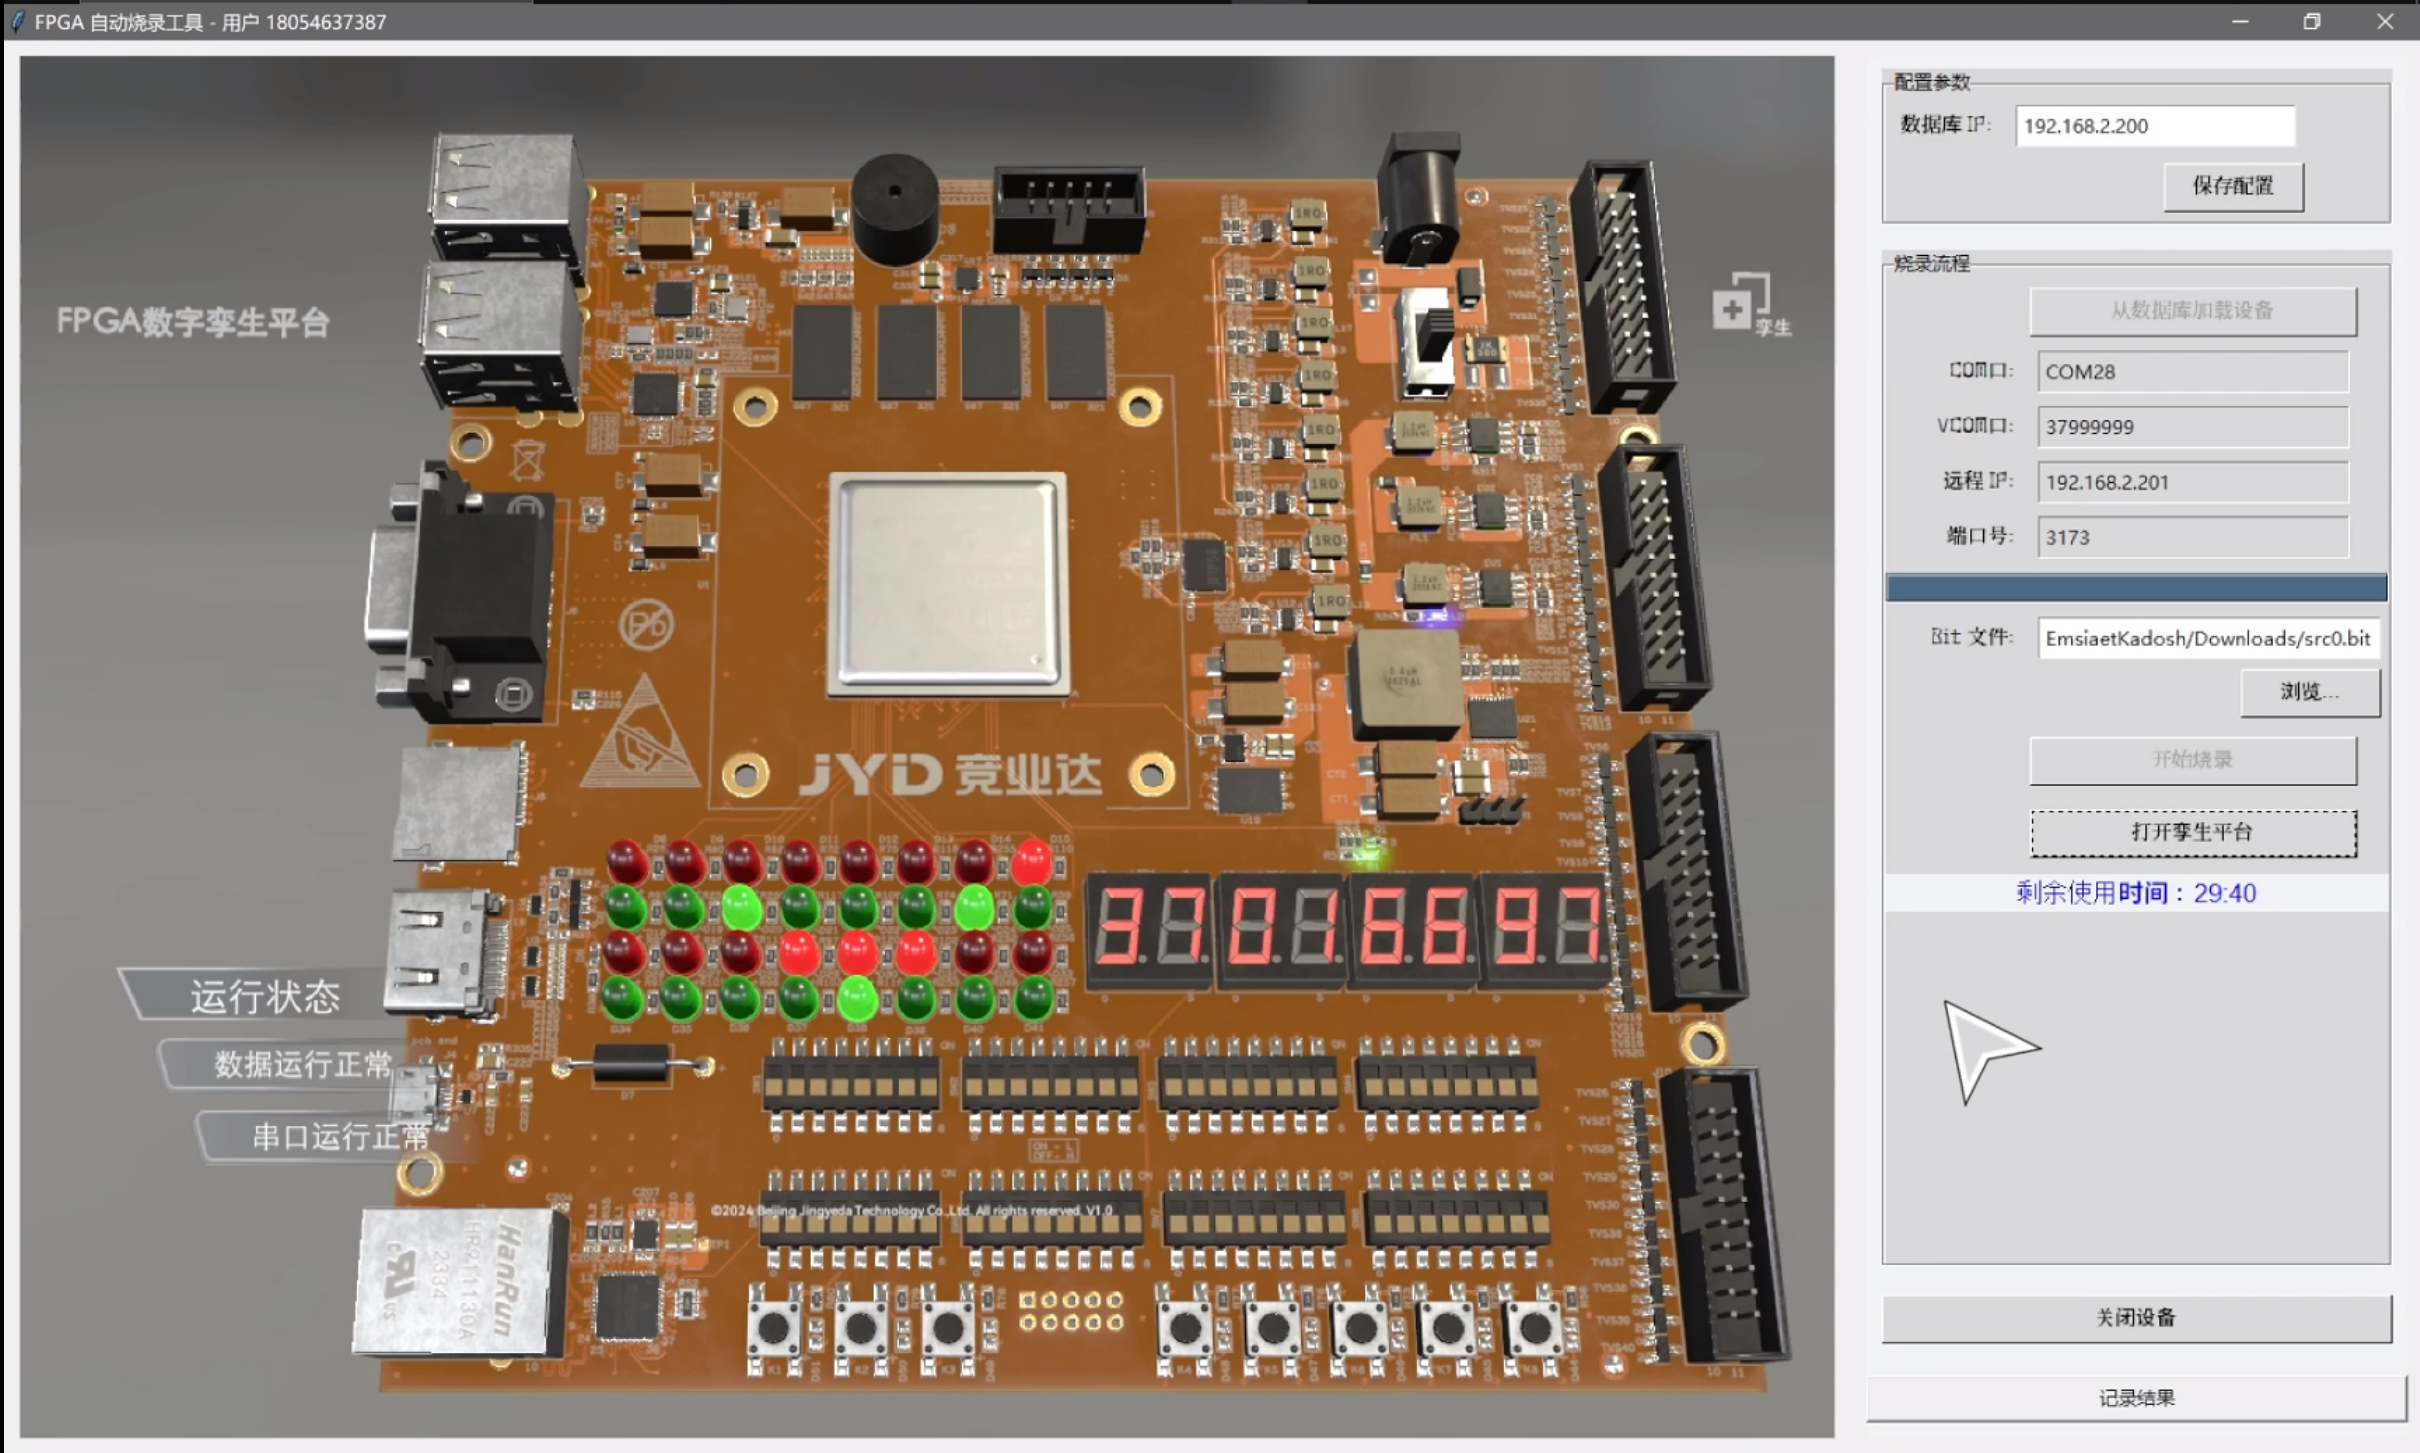
\includegraphics[width=0.8\textwidth]{src0.png}
	\caption{\code{src0.bit} 上板验证结果：RV32I 指令集测试通过 37/37，性能测试显示 \code{016697} ms，即 16.697 s。}
\end{figure}

\begin{figure}[H]
	\centering
	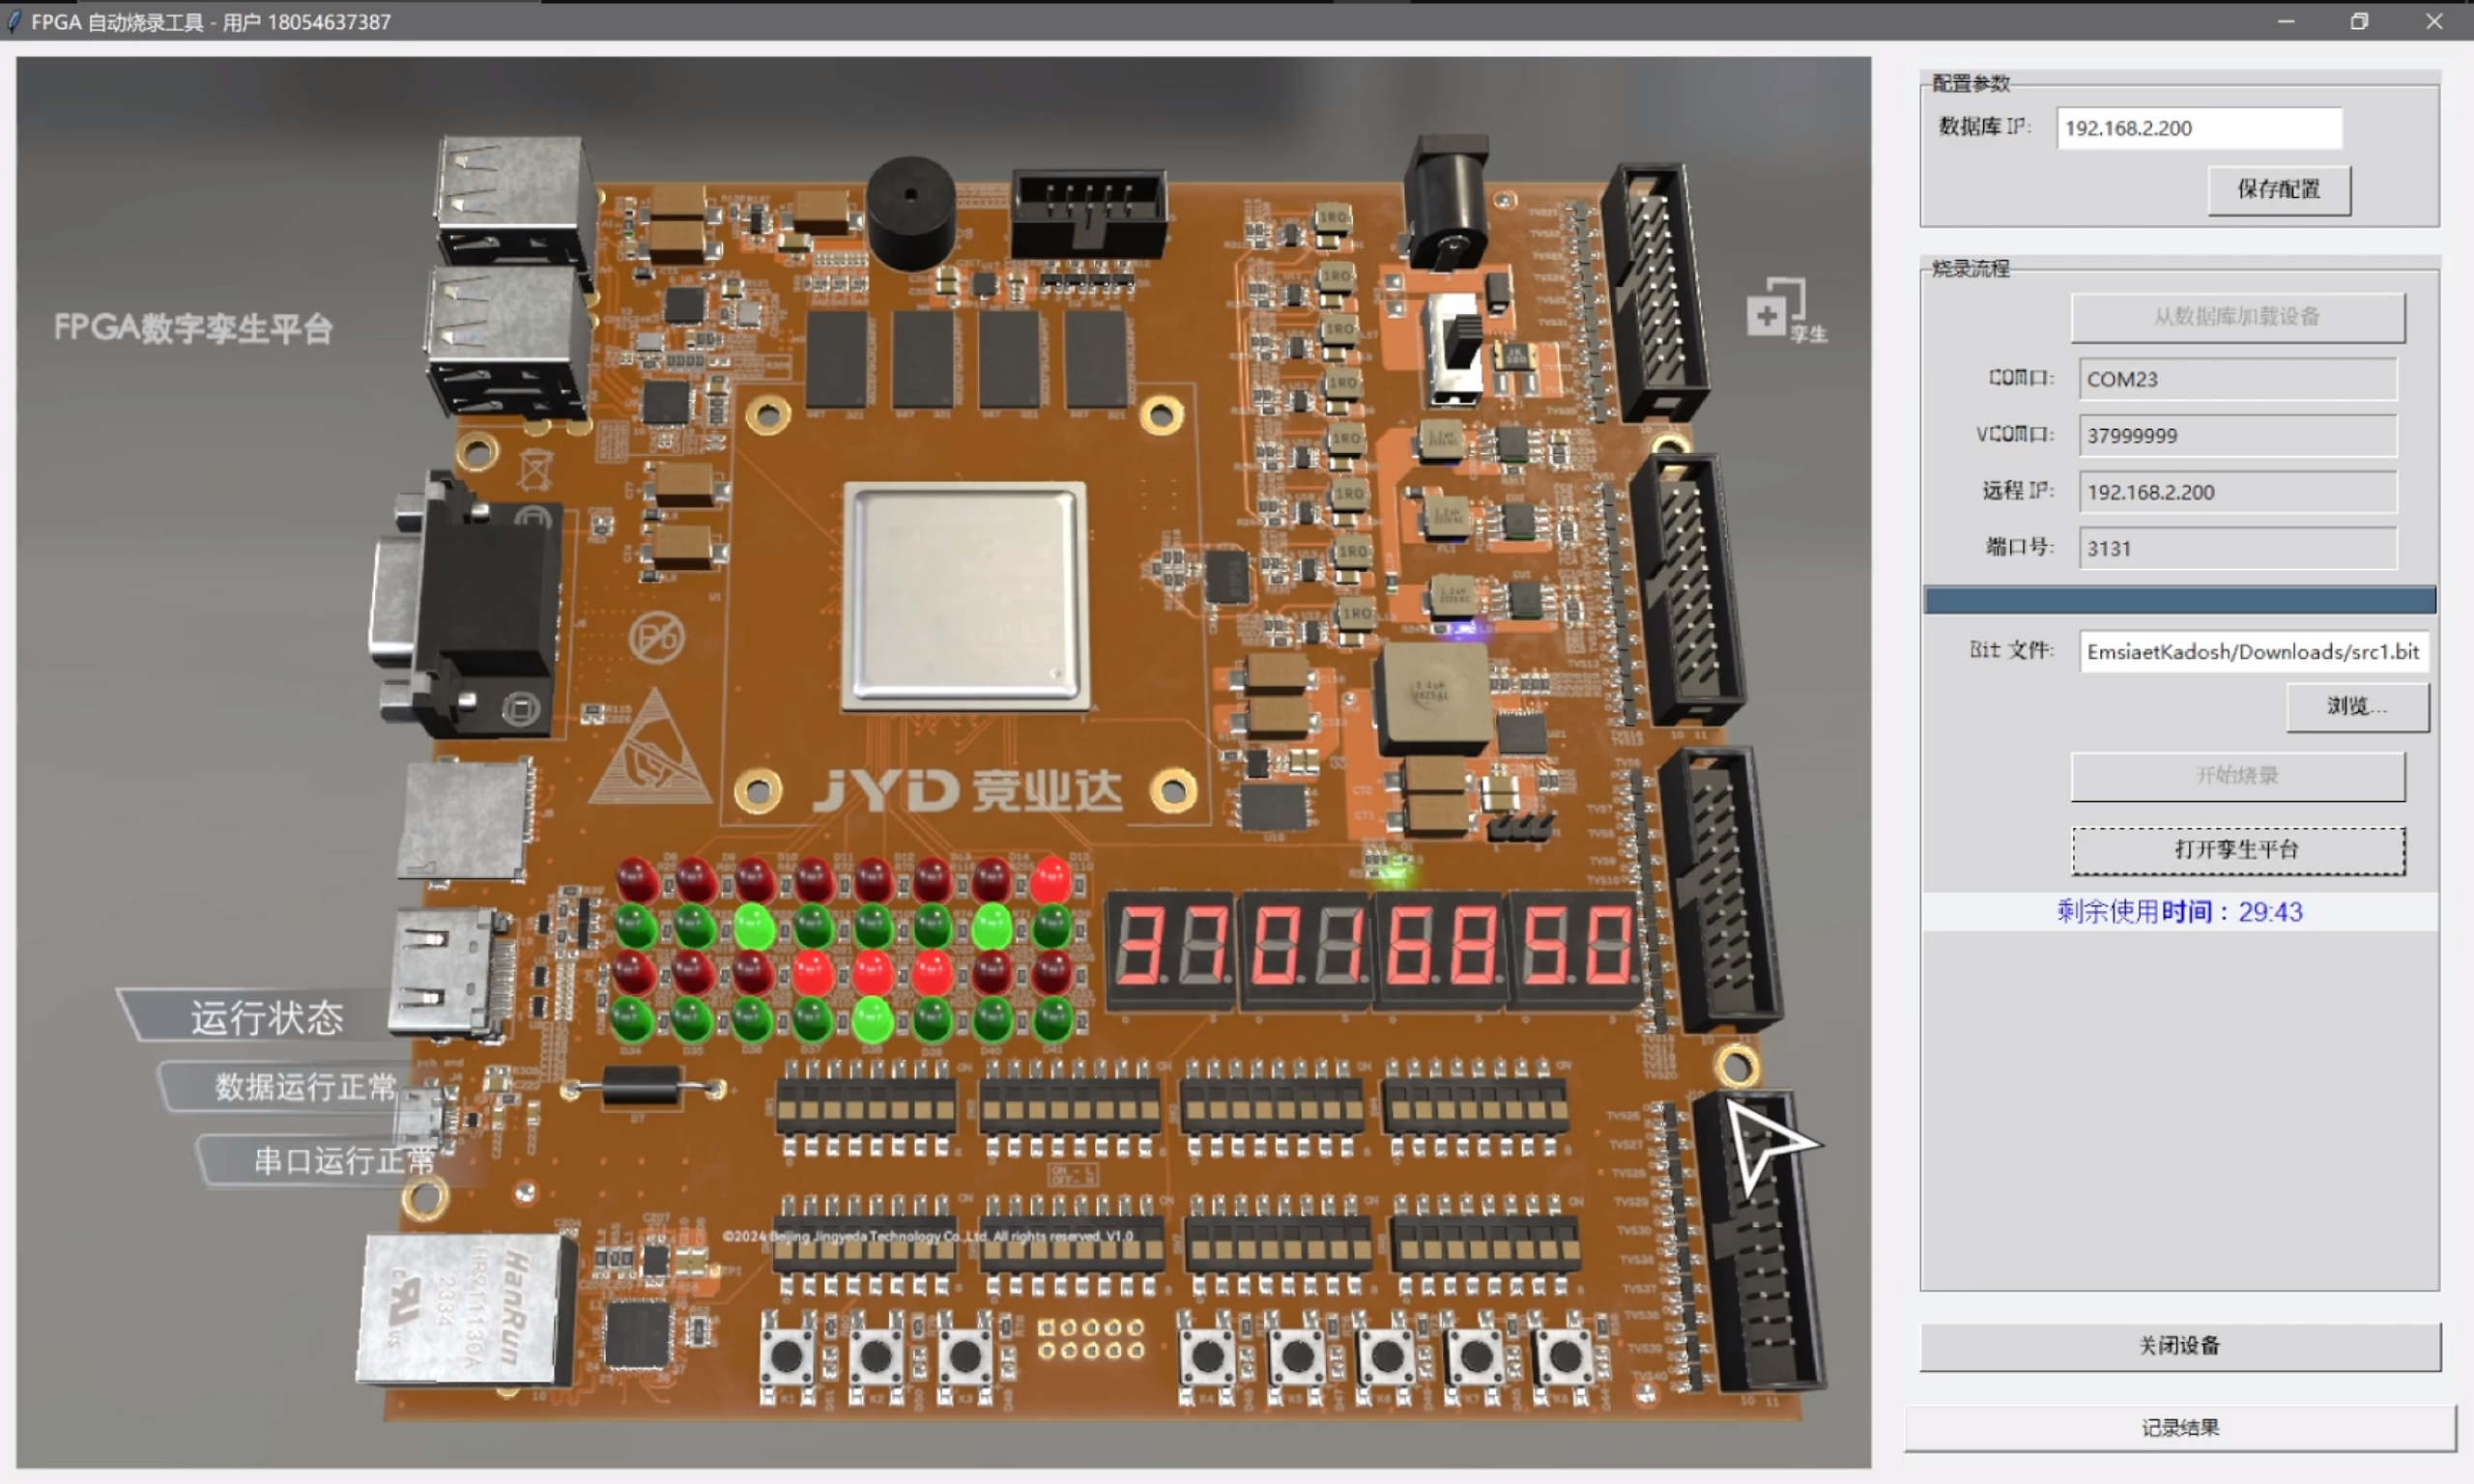
\includegraphics[width=0.8\textwidth]{src1.png}
	\caption{\code{src1.bit} 上板验证结果：RV32I 指令集测试通过 37/37，性能测试显示 \code{016850} ms，即 16.850 s。}
\end{figure}

\begin{figure}[H]
	\centering
	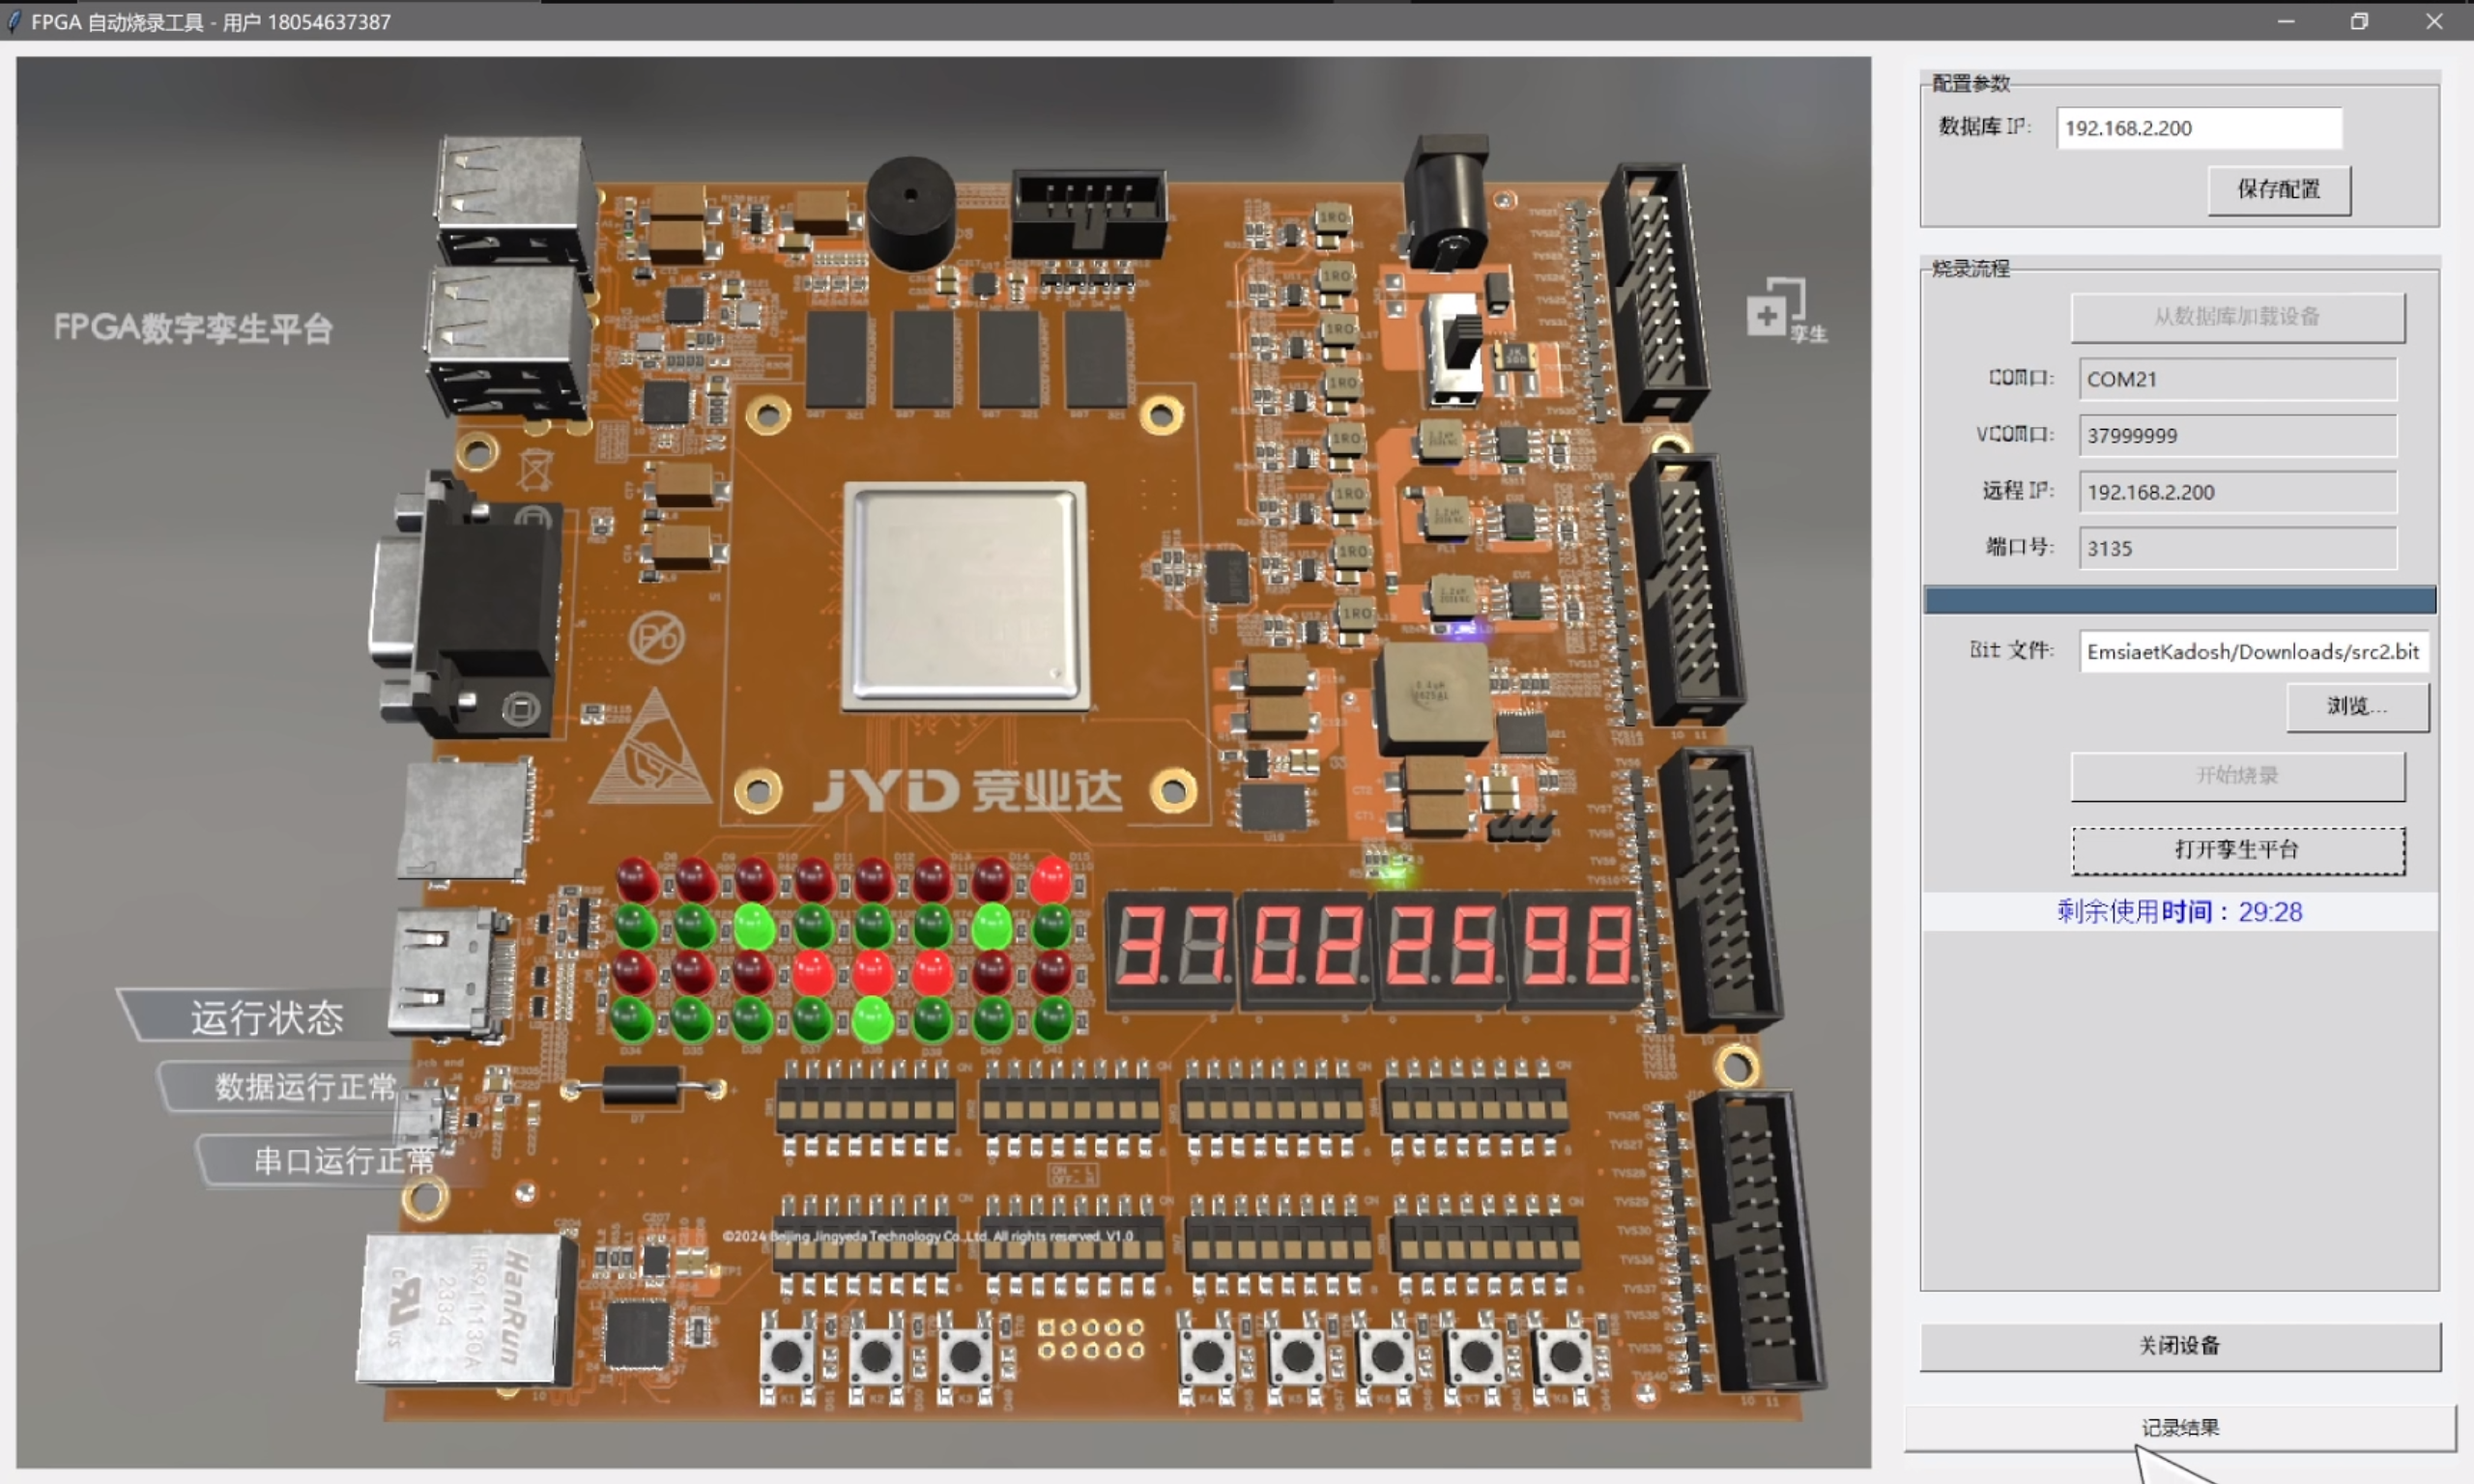
\includegraphics[width=0.8\textwidth]{src2.png}
	\caption{\code{src2.bit} 上板验证结果：RV32I 指令集测试通过 37/37，性能测试显示 \code{022598} ms，即 22.598 s。}
\end{figure}

\subsection{验证结果总结}
\begin{itemize}
	\item \textbf{指令功能测试}：三组 bit 文件的七段数码管左两位均显示 \code{37}，说明自研 CPU 已通过初赛要求的 37 条 RV32I 基础指令测试，覆盖 R 型、I 型、Load、Store、Branch、U 型和 J 型指令。测试过程中未出现 CPU 跑飞、无法显示结果或停留在异常状态的现象。
	\item \textbf{性能测试}：三组 bit 文件均能够进入并完成后续性能测试，七段数码管右六位均给出有效毫秒级计数结果。其中 \code{src0.bit} 用时 16697 ms，\code{src1.bit} 用时 16850 ms，\code{src2.bit} 用时 22598 ms。
	\item \textbf{外设交互}：板上结果表明 IROM 取指、DRAM/外设统一访问、LED 状态显示、七段数码管结果显示和计数器读写均能配合测试程序正常工作。平台界面同时显示“数据运行正常”和“串口运行正常”，说明上板通信链路与结果回传稳定。
	\item \textbf{时序验证结果}：Vivado 实现后的 Timing Summary 显示 setup、hold 和 pulse width 三类时序检查均满足约束。其中 WNS 为 0.211 ns，TNS 为 0 ns，setup failing endpoints 为 0；WHS 为 0.041 ns，THS 为 0 ns，hold failing endpoints 为 0；WPWS 为 1.100 ns，TPWS 为 0 ns，pulse width failing endpoints 为 0。该结果说明当前实现版本在目标约束下不存在 setup/hold/pulse width 时序违例，为上板稳定运行提供了时序基础。
	      \begin{figure}[H]
		      \centering
		      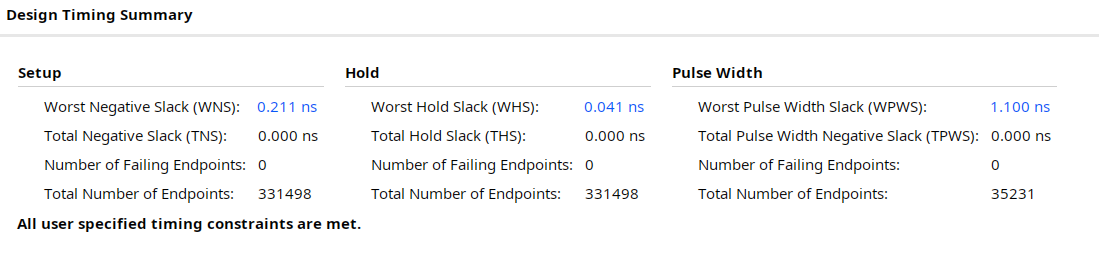
\includegraphics[width=0.8\textwidth]{timing.png}
		      \caption{Vivado 实现后 Timing Summary：WNS 为 0.211 ns，TNS 为 0 ns，WHS 为 0.041 ns，WPWS 为 1.100 ns，所有用户指定时序约束均满足。}
	      \end{figure}
	\item \textbf{综合结论}：本自研 RV32I 五级流水线 CPU 已在竞业达数字孪生平台完成三组 COE 程序上板验证。功能方面，三组测试均达到 37/37 条指令通过；性能方面，三组测试均输出有效运行时间，且 \code{src0.bit} 取得 16.697 s 的最佳板上结果；工程方面，Vivado 实现无时序违例，平台通信和外设显示稳定。因此，当前 CPU 版本不仅满足初赛上板验证的基本要求，也体现出较好的工程完整性和可重复验证能力。

\end{itemize}

\end{document}
